\title{Assignment 1: CS 763}
\author{
  Sai Charith \\ 160050083
  \and
  Sanchit Jain\\ 160050043  
  \and
  Mayank Singhal\\ 160050039 
}

\documentclass[a4paper]{article}
\usepackage{amsmath}

\usepackage{amsfonts,amssymb,amsthm}
\usepackage[margin=0.94in]{geometry}
\usepackage{graphicx}
\begin{document}
\maketitle
%\makebox[\linewidth]{\rule{\paperwidth}{0.4pt}}
%\noindent\rule{12cm}{0.4pt}
\hrulefill




\textbf{\newline Problem 3:}

\begin{figure}[ht!]
 \centering
\caption{Picture with pixel values}
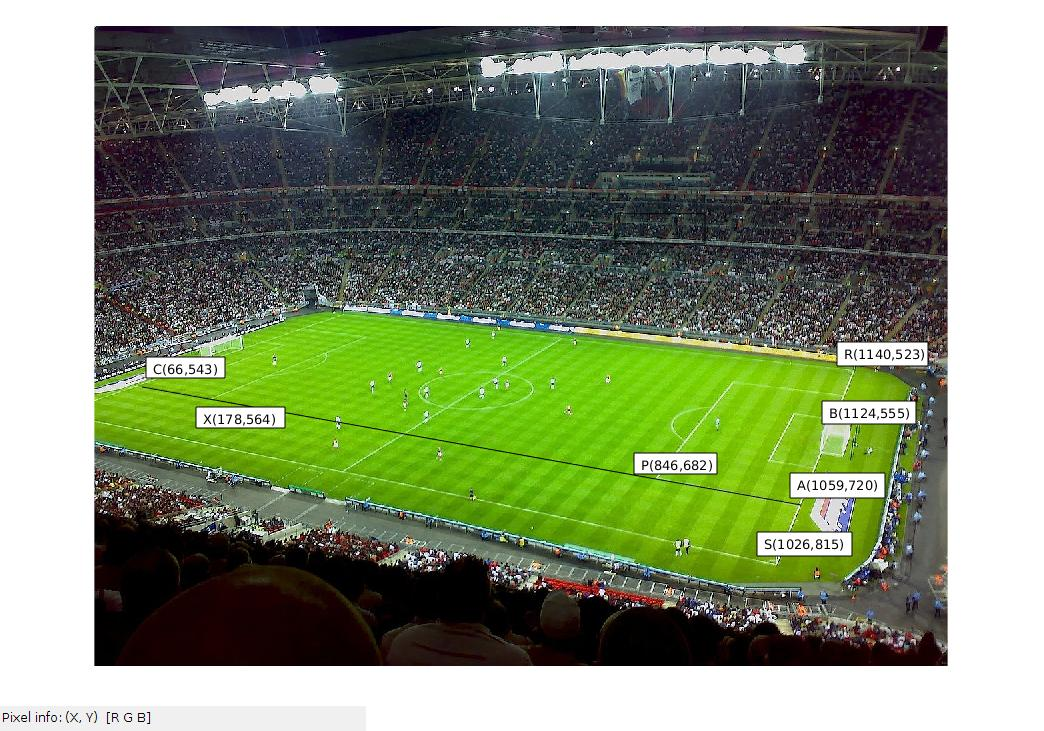
\includegraphics[width=1\textwidth]{Q2/input/measured.jpg}
\end{figure}

Let G' denote point in the real world corresponding to G in the image, 
 Using cross ratios we have 

\begin{equation*} 
\begin{split}
 \frac{AX*PC}{AC*PX} &= \frac{A'X'*P'C'}{A'C'*P'X'} \\
\ &= \frac{(A'P'+P'X')*(P'X'+X'C')}{(A'P'+P'X'+X'C')*(P'X')} \\
 \end{split}
\end{equation*}

Using pixel values from image and using symmetry of football field (ie $A'P' = X'C' = 18$ yards) and replacing $P'C'$ by $x$ we have

\begin{equation*} 
\begin{split}
\implies & 1.036 = \frac{(18+x)*(x+18)}{(18+x+18)*x}\\
\implies & x = 78.5\\
\therefore \quad & A'X' = 18+x+18 \\
\implies & A'X' =  114.5 \quad (length \; of \; field)\\
 \end{split}
\end{equation*}

Similarly
\begin{equation*} 
\begin{split}
 \frac{SB*AR}{SR*AB} &= \frac{S'B'*A'R'}{S'R'*A'B'} \\
\ &= \frac{(S'A'+A'B')*(A'B'+B'R')}{(S'A'+A'B'+B'R')*(A'B')} \\
 \end{split}
\end{equation*}

Using pixel values from image and using symmetry of football field (ie $S'A' = B'R'$) and replaicing $S'A',B'R'$ by $x$  we have

\begin{equation*} 
\begin{split}
\implies & 1.07 = \frac{(x+44)*(44+x)}{(44+2x)*44}\\
\implies & x = 14.7\\
\because \quad & S'R' = x+44+x \\
\implies & S'R' = 73.4 \quad (length \; of \; field)\\
 \end{split}
\end{equation*}

So, the dimensions of the pitch are $114.5 \times 73.4$

The above method uses symmtry of football field (i.e both Dees have same dimemsions. The dimensions of the field can also be calculated by calculating the vanishing points along AP and AB (using point of intersection of parallel lines) and using cross ratios. But the lines in the image are almost parellel so there would be lot of error in calculating points of intersection. Hence we preffered using symmetry in the field.

\hrulefill \\


\textbf{\newline Problem 5:}

Although there was high amount of noise in the second image the joint entropy turned out to be minimum when the images were almost aligned.

The joint entropy of an (image,constant image) is same as joint entropy of (image,image). As joint histograms take straight line shape in both cases.   


\begin{figure}[ht!]
 \centering
%\caption{Picture with pixel values}
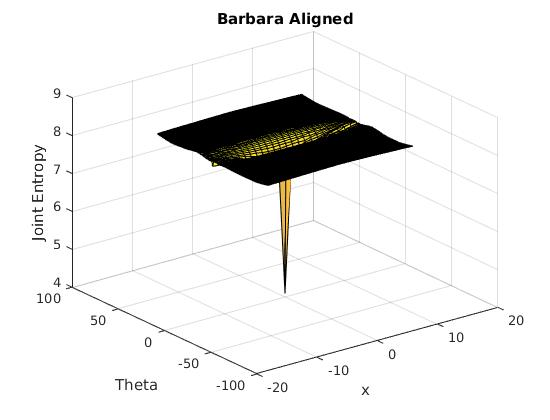
\includegraphics[width=0.5\textwidth]{Q5/output/barbara_je.jpg}
\end{figure}
\begin{figure}[ht!]
 \centering
%\caption{Picture with pixel values}
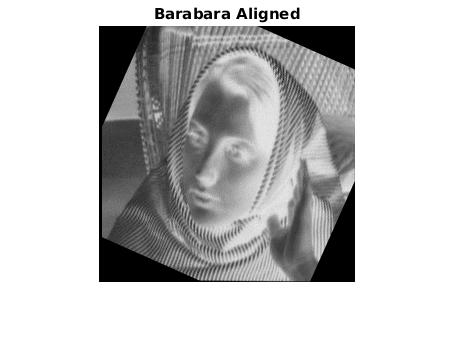
\includegraphics[width=0.75\textwidth]{Q5/output/Barbara_aligned.jpg}
\end{figure}
\begin{figure}[ht!]
 \centering
%\caption{Picture with pixel values}
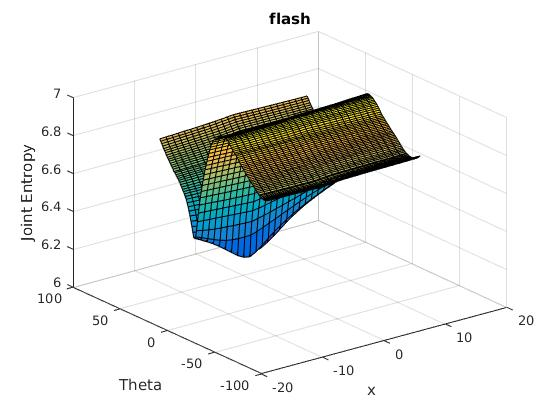
\includegraphics[width=0.5\textwidth]{Q5/output/noflash_je.jpg}
\end{figure}
\begin{figure}[ht!]
 \centering
%\caption{Picture with pixel values}
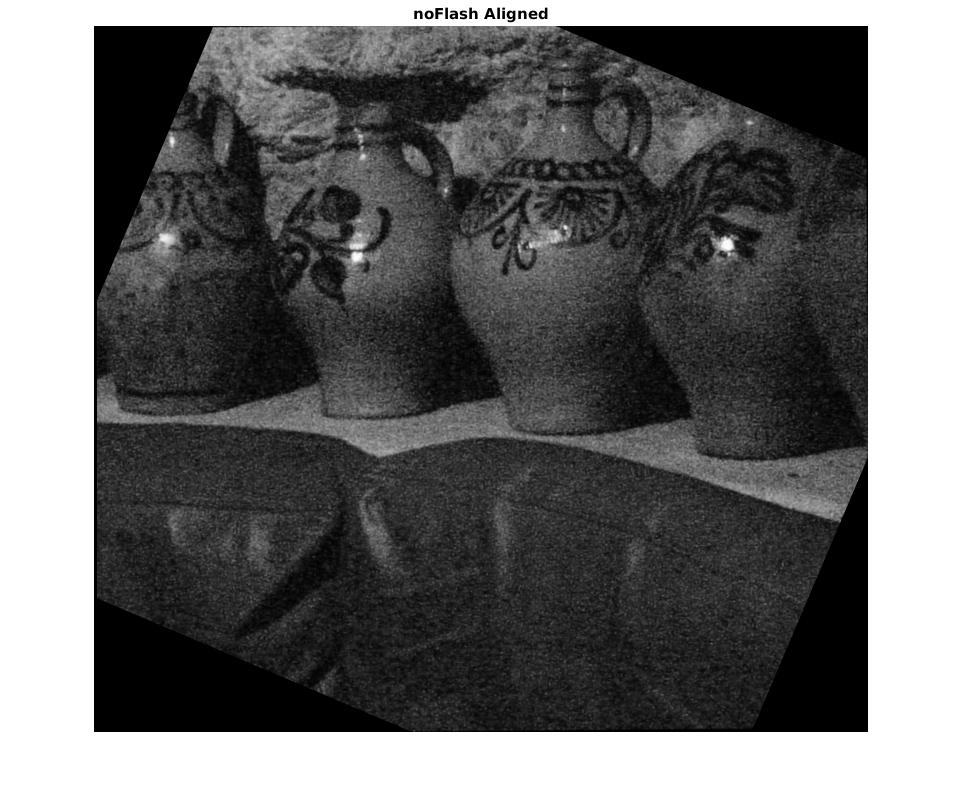
\includegraphics[width=0.75\textwidth]{Q5/output/noflash_aligned.jpg}
\end{figure}
\begin{figure}[ht!]
 \centering
%\caption{Picture with pixel values}
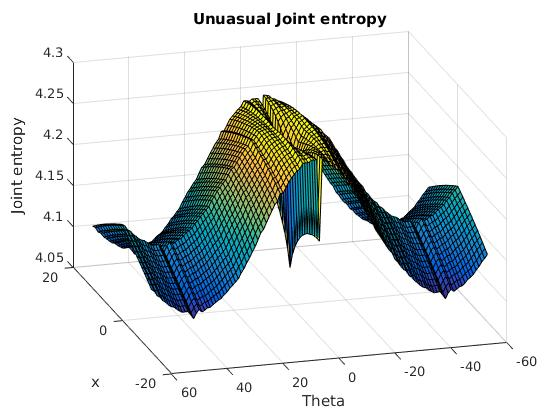
\includegraphics[width=0.5\textwidth]{Q5/output/unusual.jpg}
\end{figure}




\end{document}
